\pdfminorversion=4
\documentclass[aspectratio=169]{beamer}

\mode<presentation>
{
  \usetheme{default}
  \usecolortheme{default}
  \usefonttheme{default}
  \setbeamertemplate{navigation symbols}{}
  \setbeamertemplate{caption}[numbered]
  \setbeamertemplate{footline}[frame number]  % or "page number"
  \setbeamercolor{frametitle}{fg=white}
  \setbeamercolor{footline}{fg=black}
} 

\usepackage[english]{babel}
\usepackage[utf8x]{inputenc}
\usepackage{tikz}
\usepackage{courier}
\usepackage{array}
\usepackage{bold-extra}
\usepackage{minted}
\usepackage[thicklines]{cancel}
\usepackage{fancyvrb}

\xdefinecolor{dianablue}{rgb}{0.18,0.24,0.31}
\xdefinecolor{darkblue}{rgb}{0.1,0.1,0.7}
\xdefinecolor{darkgreen}{rgb}{0,0.5,0}
\xdefinecolor{darkgrey}{rgb}{0.35,0.35,0.35}
\xdefinecolor{darkorange}{rgb}{0.8,0.5,0}
\xdefinecolor{darkred}{rgb}{0.7,0,0}
\definecolor{darkgreen}{rgb}{0,0.6,0}
\definecolor{mauve}{rgb}{0.58,0,0.82}

\title[2020-08-11-snowmass-github]{{\LARGE 5 plots in 5 minutes:} \\ Using GitHub API to measure software adoption in CMS}
\author{Jim Pivarski}
\institute{Princeton University -- IRIS-HEP}
\date{August 11, 2020}

\usetikzlibrary{shapes.callouts}

\begin{document}

\logo{\pgfputat{\pgfxy(0.11, 7.4)}{\pgfbox[right,base]{\tikz{\filldraw[fill=dianablue, draw=none] (0 cm, 0 cm) rectangle (50 cm, 1 cm);}\mbox{\hspace{-8 cm}
\includegraphics[height=1 cm]{princeton-logo-long.png}\hspace{0.1 cm}\raisebox{0.1 cm}{
\includegraphics[height=0.8 cm]{iris-hep-logo-long.png}}\hspace{0.1 cm}}}}}

\begin{frame}
  \titlepage
\end{frame}

\logo{\pgfputat{\pgfxy(0.11, 7.4)}{\pgfbox[right,base]{\tikz{\filldraw[fill=dianablue, draw=none] (0 cm, 0 cm) rectangle (50 cm, 1 cm);}\mbox{\hspace{-8 cm}
\includegraphics[height=1 cm]{princeton-logo.png}\hspace{0.1 cm}\raisebox{0.1 cm}{
\includegraphics[height=0.8 cm]{iris-hep-logo.png}}\hspace{0.1 cm}}}}}

% Uncomment these lines for an automatically generated outline.
%\begin{frame}{Outline}
%  \tableofcontents
%\end{frame}

% START START START START START START START START START START START START START

\begin{frame}{Goal: find out how physicists are using software for data analysis}
\Large

\vspace{0.5 cm}
Workflow from detector $\to$ reconstruction $\to$ AODs is understood.

\vspace{0.5 cm}
Workflow from AODs $\to$ analysis $\to$ proposed papers is not.

\vspace{0.5 cm}
\begin{itemize}
\item Distributed collaboration: who is even doing the work?
\item Awareness of and response to surveys is uneven.
\item Can we get a more direct method?
\end{itemize}
\end{frame}

\begin{frame}{Method: look at their code!}
\Large

\vspace{0.5 cm}
GitHub API gives us programmatic statistics (URL $\to$ JSON) on users and their repositories.

\vspace{0.5 cm}
But first we have to identify ``physicists.''
\large

\vspace{0.5 cm}
\begin{itemize}
\item CMSSW has been on GitHub since 2013; fork-and-pull request is how CMS physicists contribute.
\item Assumption: high correlation between forking CMSSW and CMS physicists.
\item The same users do their own work in non-fork repositories.
\item Why CMS/GitHub? Until recently, all (free) GitHub repos were public, and only public repos can be analyzed. In GitLab, many repos are private.
\end{itemize}

\vspace{0.25 cm}
Large dataset: \textcolor{darkorange}{\bf 3100 users} with \textcolor{darkorange}{\bf 19\,400 non-fork repos} spanning \textcolor{darkorange}{\bf 7 years}.
\end{frame}

\begin{frame}{Plot \#1: language choice}
\vspace{0.25 cm}
Using GitHub's algorithm for determining a repo's programming language.

\vspace{0.15 cm}
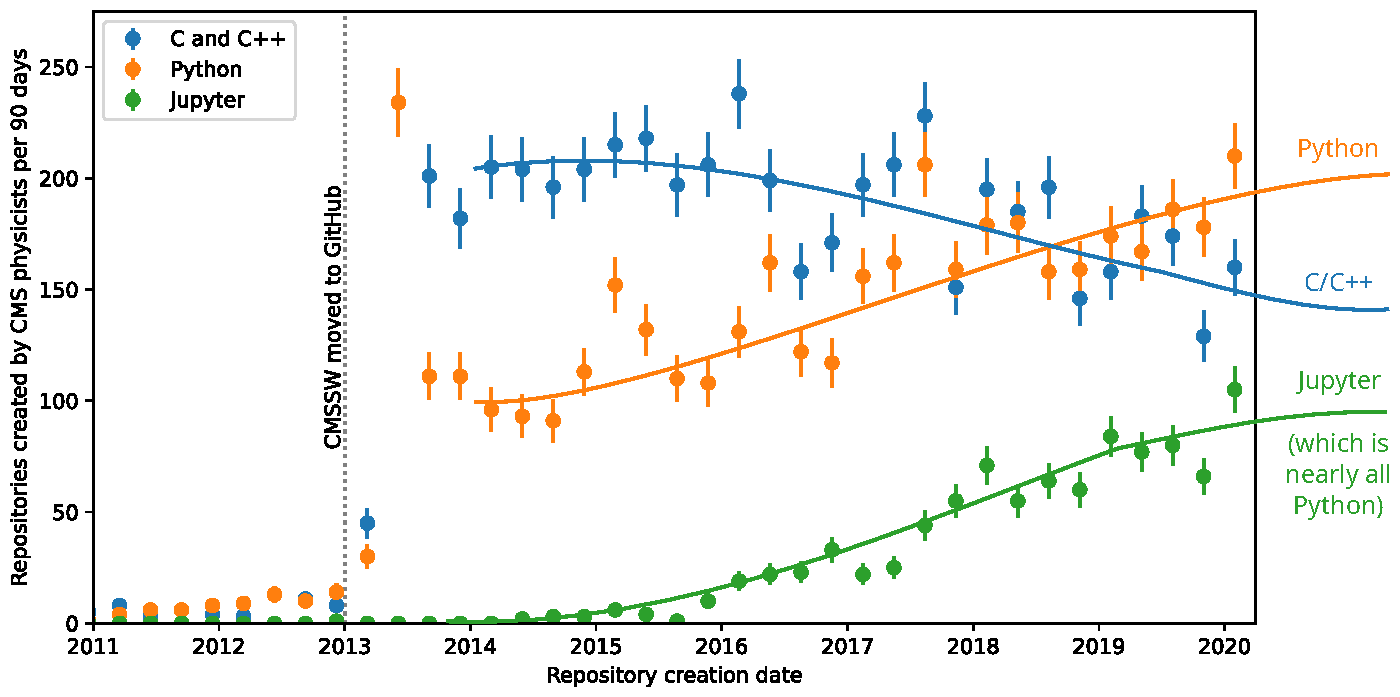
\includegraphics[width=\linewidth]{01-github-cmssw-language.pdf}
\end{frame}

\begin{frame}{Plot \#2: language choice by user}
\vspace{0.25 cm}
Same thing, but with average number of repos per user instead of total repos.

\vspace{0.15 cm}
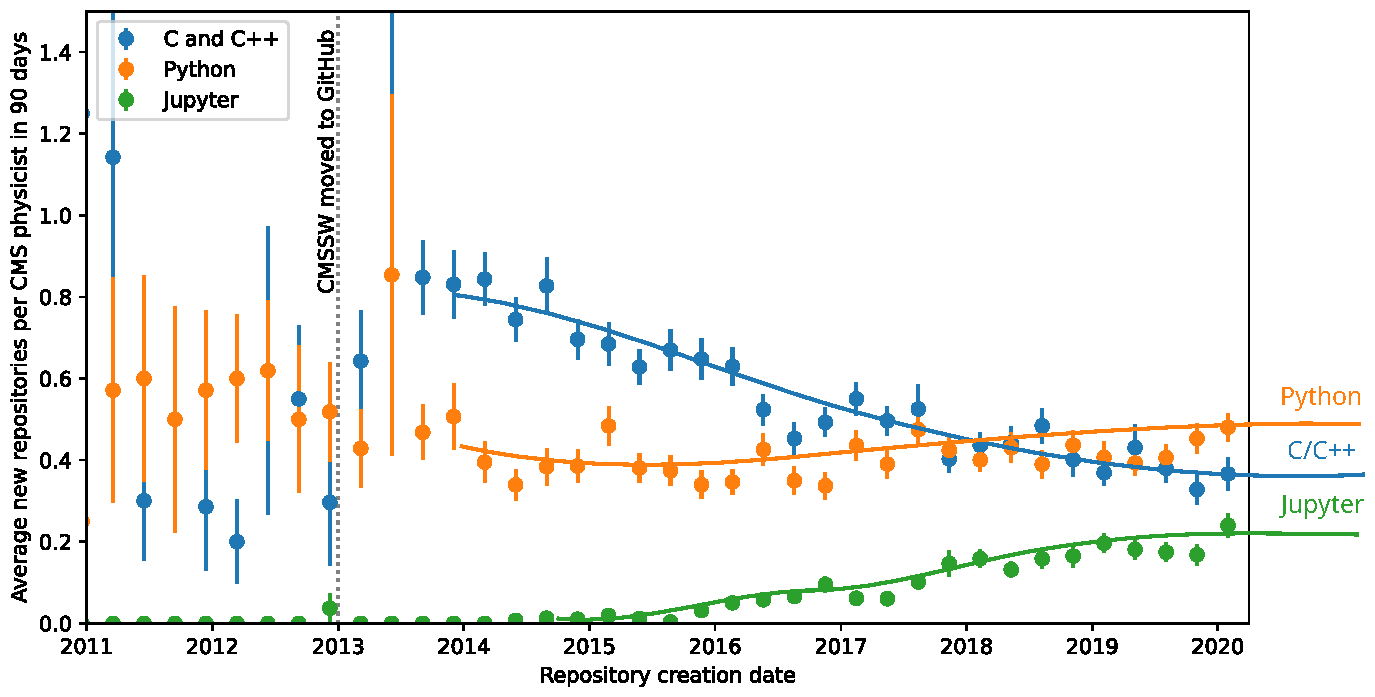
\includegraphics[width=\linewidth]{02-github-cmssw-language-byuser.pdf}
\end{frame}

\begin{frame}{Plot \#3: search for package imports}
\vspace{0.25 cm}
Number of repos that match a search string (within C/C++ or Python/Jupyter files).

\vspace{0.15 cm}
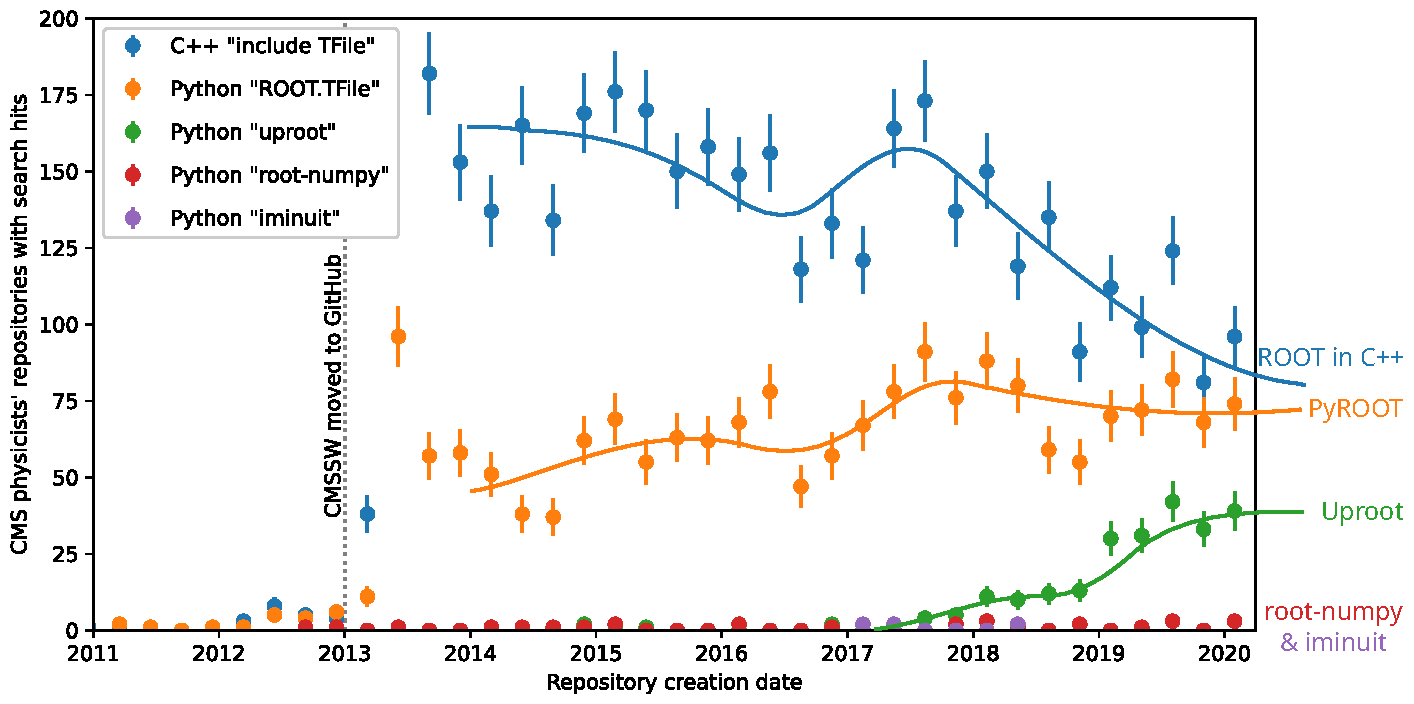
\includegraphics[width=\linewidth]{03-github-root-python.pdf}
\end{frame}

\begin{frame}{Plot \#4: what machine learning packages do they use?}
\vspace{0.25 cm}
Same technique. Dominance of Scikit-Learn (over TensorFlow and Torch) is surprising.

\vspace{0.15 cm}
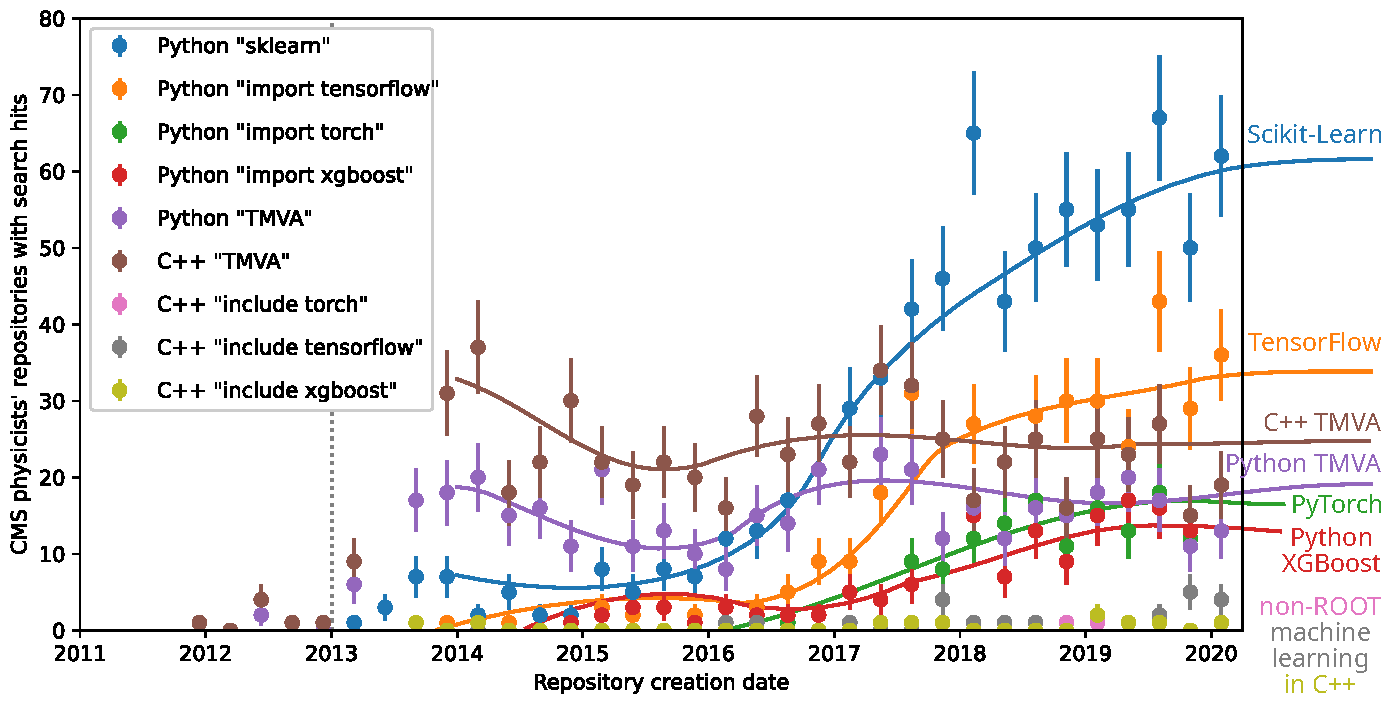
\includegraphics[width=\linewidth]{04-github-machine-learning.pdf}
\end{frame}

\begin{frame}{Plot \#5: Did machine learning drive Python adoption?}
\vspace{0.25 cm}
Not really. Basic analysis tools (NumPy, Matplotlib, Pandas) outweigh Pythonic ML.

\vspace{0.15 cm}
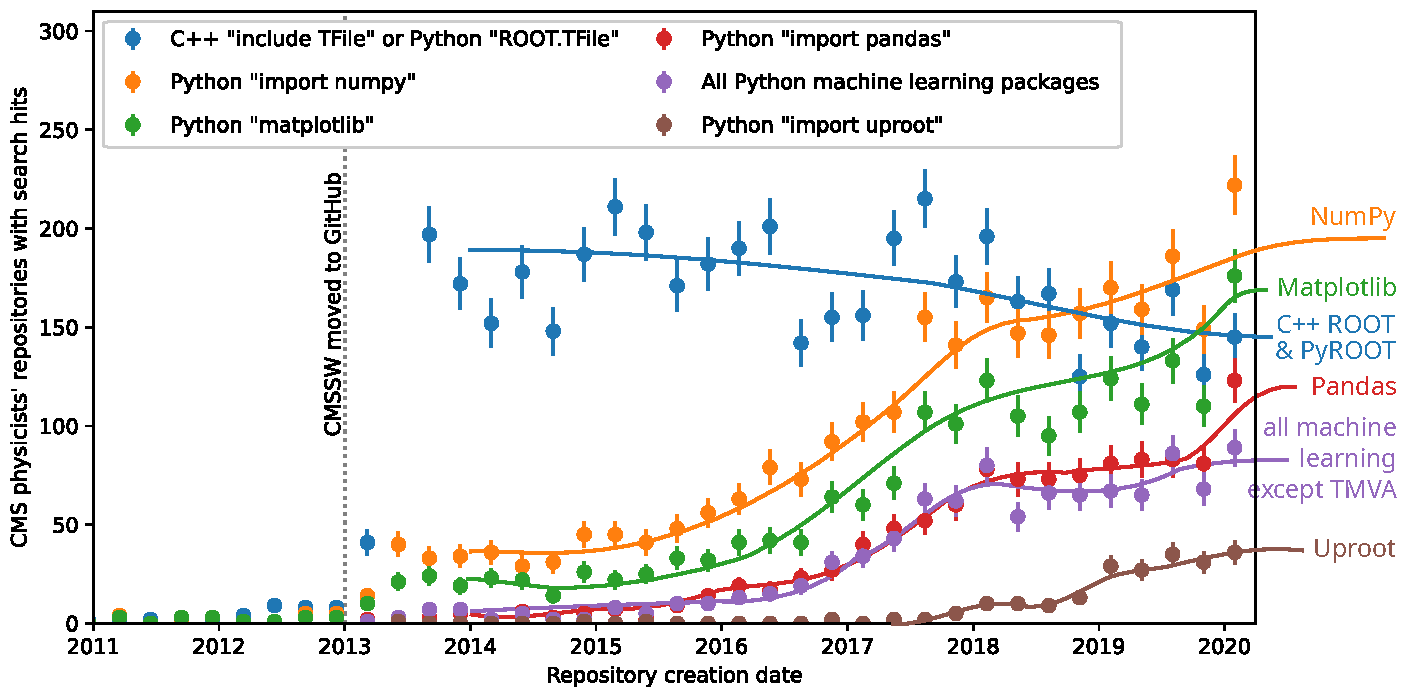
\includegraphics[width=\linewidth]{05-github-anyroot-python-machinelearning-uproot.pdf}
\end{frame}

\end{document}
